Diff eqs:-
  \item Scholarship 2015: A tank contains 200 litres of brine (solution of salt in water). Initially, the concentration is \SI{0.5}{\kilo\gram}
        of salt per litre. Brine containing \SI{0.8}{\kilo\gram} of salt per litre runs into the tank at a rate of 6 litres per
        minute. The mixture is kept thoroughly mixed and is running out at the same rate.

        Find out how long it takes for the amount of salt in the tank to be \SI{130}{\kilo\gram}.
  \question The \textit{logistic equation} is used when modelling populations:
            \begin{displaymath}
              \od{P}{t} = rP(1-P)
            \end{displaymath}
    \begin{parts}
      \part Find $ P(t) $ explicitly.
      \part Examine the behaviour of the population as $ t \to \infty $. Graph the function.
      \part Examine the behaviour of the population over time if you vary $ r $ (check $ r = 0 $, and $ r < 0 $ for example).
      \part Do you think the logistic equation is a good model? Why/why not?
    \end{parts}
  \questioS Solve the following differential equation for $ y(x) $:
    \begin{displaymath}
      \od{y}{x} = \frac{y^2 - a^4}{x^2 - a^2}
    \end{displaymath}
  \questioS Scholarship 2008:
    \begin{parts}
      \part $ \dfrac{A}{x} + \dfrac{B}{P-x} = \dfrac{1}{x(P-x)} $ where $ x $ is a variable and $ P $ is a constant.
            Find $ A $ and $ B $ in terms of $ P $.
      \part When a rumour about a teacher is started at a school of size $ P $ students, it spreads at a rate (in students
            per day) that is proportional to the product of the number of students who know the rumour, $ N $, and those who
            do not. Find an expression for the number of students $ N $ who know the rumour after $ t $ days.
      \part For a particular rumour about a teacher, 0.5\% of students know the rumour initially. The principal will need to act
            to stop the rumour once more than half the school's students know it. When $ \dfrac{1}{5} $ of the students know the
            rumour, the number who know the rumour is increasing at a rate of $ 0.08P $ students per day.
            How long will it be before the principal must act?
    \end{parts}
  \questioO Scholarship 2015: The rate of spread of a rumour at a particular school is proportional to both
            the number of students who know a rumour, $ S $, and the number of students who do not.
            If $ N $ is the total number of students in the school, then $ \od{S}{t} = kS(N-S) $.
            Initially, two students knew the rumour. Show that the number of students who know the
            rumour at time $ t $ is $ S(t) = \dfrac{N}{1 + \dfrac{1}{2} e^{-kNt}(N-2)} $.

def integrals:
  \questioM Compute the following definite integrals:
    \begin{parts}
      \part $ \rint^1_0 xe^{-x^2} \dif{x} $
      \part $ \rint^{\pi/3}_{-\pi/3} x^4 \sin x \dif{x} $ (hint: no substitution is required)
      \part $ \rint^1_0 \cos(\pi t/2) \dif{t} $
      \part $ \rint^1_0 (3t - 1)^{50} \dif{t} $
      \part $ \rint^1_0 \sqrt[3]{1 + 7x} \dif{x} $
      \part $ \rint^1_0 \frac{\dif{x}}{1 + \sqrt{x}} \dif{x} $
      \part $ \rint^2_{-1} x(x-1)^3 \dif{x} $
      \part $ \rint^3_0 x\sqrt{1 + x^2} \dif{x} $
    \end{parts}
  \questioM Find the area enclosed by the curve $ y = 4 \sin 3x \cos x $ and the $ x-$axis from $ x = 0 $
            to $ x = \frac{\pi}{3} $.
  \questioE Find $ k $ such that $ \rint^k_0 e^{2x} \dif{x} = 40 $.
  \questioE Calculate the area enclosed by the curve $ y = \frac{3x - 2}{x + 4} $ and the lines $ y = 0 $, $ x = 1 $,
            and $ x = 5 $.
  \questioE Find the area between the curves $ y = \sin^2 kx $ and $ y = \cos^2 kx $ shaded below.
            \begin{center}
              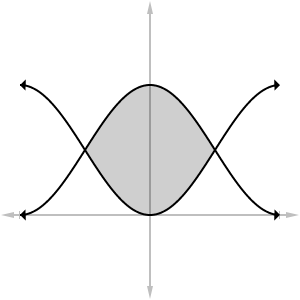
\includegraphics[width=0.3\textwidth]{int4}
            \end{center}
  \questioS Evaluate $ I = \rint^{\pi/2}_0 \frac{\sqrt{\sin x}}{\sqrt{\sin x} + \sqrt{\cos x}} \dif{x} $ [\textit{Hint: use the
            substitution $ x = \frac{\pi}{2} - u $ and add the result to the original integral.}]
